\documentclass[10pt,a4paper]{article}

% ─── Packages ─────────────────────────────────────────

\usepackage{fontspec}
\setmainfont{Times New Roman}

\usepackage[top=1.0cm,bottom=0.9cm,left=1.45cm,right=1.45cm]{geometry}

\usepackage{titlesec}
\usepackage{enumitem}
\usepackage{hyperref}
\usepackage{xcolor}
\usepackage{tabularx}
\usepackage{graphicx}
\usepackage{parskip}

% ─── Colors ───────────────────────────────────────────

\definecolor{primary}{RGB}{30,40,90}
\definecolor{namecolor}{RGB}{0,120,180}
\definecolor{accent}{RGB}{50,90,150}
\definecolor{rulecol}{RGB}{200,205,220}
\definecolor{gray}{RGB}{90,90,90}

\hypersetup{
    colorlinks=true,
    urlcolor=accent
}

\pagestyle{empty}
\setlength{\parskip}{0pt}

% ─── Section ──────────────────────────────────────────

\titleformat{\section}
    {\normalsize\bfseries\color{primary}}
    {}
    {0em}
    {}
    [\vspace{1pt}\textcolor{rulecol}{\titlerule[0.6pt]}\vspace{1pt}]

\titlespacing{\section}{0pt}{4pt}{2pt}

% ─── Entry ────────────────────────────────────────────

\newcommand{\entry}[3]{%
    \noindent
    \begin{tabularx}{\linewidth}{X r}
        \textbf{\color{primary}#1} &
        {\scriptsize\color{gray}#2}
    \end{tabularx}\\[-2pt]
    {\scriptsize\textit{\color{gray}#3}}
    \vspace{0.5pt}
}

% ─── Compact list ─────────────────────────────────────

\newenvironment{cvitems}{
    \begin{itemize}[
        leftmargin=1.1em,
        topsep=0pt,
        itemsep=0.3pt,
        parsep=0pt,
        partopsep=0pt
    ]
}{
    \end{itemize}
}

% ═════════════════════════════════════════════════════

\begin{document}

% ─── HEADER ───────────────────────────────────────────

\noindent

\begin{tabularx}{\linewidth}{@{}X r@{}}

\begin{minipage}[c]{\linewidth}

    {\LARGE\bfseries\color{namecolor} Ho Huynh Nhu}\\[1pt]

    {\large\bfseries\color{primary}
    ERP Implementation Intern}\\[2pt]

    {\scriptsize\color{gray}
    20/10/2003
    \enspace\textcolor{rulecol}{|}
    \enspace (+84) 367 503 477
    \enspace\textcolor{rulecol}{|}
    \enspace
    \href{mailto:hhnhu2003@gmail.com}{hhnhu2003@gmail.com}
    \enspace\textcolor{rulecol}{|}
    \enspace Ho Chi Minh City}\\[1pt]

    {\scriptsize
    \href{https://github.com/hohuynhnhu}
    {github.com/hohuynhnhu}
    \enspace\textcolor{rulecol}{|}
    \enspace
    \href{https://www.facebook.com/huynhnhu.ho.961}
    {facebook.com/huynhnhu.ho.961}
    }

\end{minipage}

&

\begin{minipage}[c]{2.1cm}
    \raggedleft
    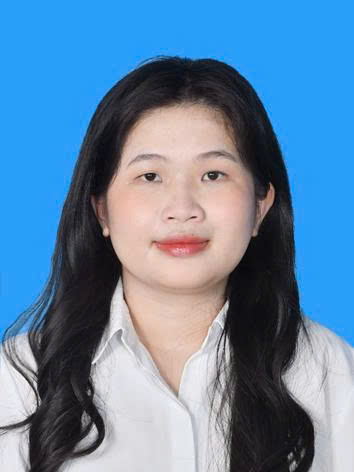
\includegraphics[
        width=2.1cm,
        height=2.5cm,
        keepaspectratio
    ]{assets/avt.jpg}
\end{minipage}

\end{tabularx}

\vspace{2pt}

\textcolor{rulecol}{\rule{\linewidth}{0.6pt}}

% ─── CAREER OBJECTIVE ─────────────────────────────────

\section*{Career Objective}

{\small
Final-year Information Technology student seeking an internship in ERP
implementation and operations. Experienced in working with business data from
the Odoo ERP system (extraction, standardization, reporting), automating data
workflows, integrating systems through APIs, and building Power BI reports
to monitor operations. Experienced in teamwork using Jira and Confluence,
and eager to learn and contribute to requirement analysis, process setup,
progress tracking, and risk control in ERP projects.
}

% ─── EDUCATION ────────────────────────────────────────

\section*{Education}

\entry
{University of Transport Ho Chi Minh City (UTH)}
{10/2022 -- 10/2026}
{Bachelor of Information Technology -- Completed coursework}

{\small
\begin{cvitems}

    \item GPA: \textbf{3.4 / 4.0}

    \item \textbf{Excellent Scholarship} -- Semester 1, 2025

    \item \textbf{Second Prize -- AI Track},
    UTH Student Scientific Research Conference 2025

\end{cvitems}
}

% ─── TECHNICAL SKILLS ─────────────────────────────────

\section*{Technical Skills}

{\small

\begin{tabularx}{\linewidth}{@{}lX@{}}

\textbf{ERP \& Business Process}
&
Odoo (business data), Process Analysis through Data,
Workflow Automation (Power Apps, SharePoint), Process Documentation
\\[1pt]

\textbf{System Integration}
&
RESTful API, FastAPI, Postman, Microservices, RabbitMQ, Kafka
\\[1pt]

\textbf{SQL / Databases}
&
SQL, PostgreSQL, SQL Server, MySQL, Joins, Aggregations,
MongoDB, Firebase, Supabase
\\[1pt]

\textbf{BI / Reporting}
&
Power BI, DAX, Excel, Operational Reporting, KPI Analysis
\\[1pt]

\textbf{ETL / Automation}
&
Python, ETL/ELT, dbt, Apache Airflow, Data Pipeline, Data Warehouse
\\[1pt]

\textbf{Project Management \& Collaboration}
&
Jira, Confluence, Git, Project Progress Reporting

\end{tabularx}

}

% ─── WORK EXPERIENCE ──────────────────────────────────

\section*{Work Experience}

\entry
{Gotik Consulting -- Data Engineer}
{Python \textbar{} dbt \textbar{} PostgreSQL \textbar{} Airflow \textbar{} Power BI}
{03/2026 -- 05/2026}

{\small
\begin{cvitems}
    \item Worked with business data from the Odoo ERP system: extracted, cleaned, and standardized data using Python and SQL to prepare structured datasets for analytics and reporting.

    \item Built ETL pipelines to load data from source systems into Neon PostgreSQL and automated hourly runs with Apache Airflow, keeping data up to date and running continuously.

    \item Monitored ETL runs (schedules, task dependencies, failures) to detect and resolve incidents and keep the system stable.

    \item Developed dbt models to standardize raw data, improving consistency and making reporting processes easier to maintain and reuse.

    \item Built Power BI dashboards to track operational and business metrics, supporting performance evaluation and decision-making.
\end{cvitems}
}

% ─── PROJECTS ─────────────────────────────────────────

\section*{Featured Projects}

\entry
{Delivery Driver -- Order Management \& Analytics System}
{Python \textbar{} PostgreSQL \textbar{} Kafka \textbar{} MinIO \textbar{} RFM \textbar{} Association Rule Mining}
{12/2025 -- 02/2026}

{\small
\begin{cvitems}
    \item Built an automated data pipeline with a Data Lake and Data Warehouse to collect and process order data in real time.
    \item Applied RFM and Association Rule Mining to analyze orders and frequent pickup--delivery location pairs, generating insights to support recommendations for opening new post offices or service points.
    \item GitHub: \href{https://github.com/LeKhang-cn22h/BE-delivery-driver}{BE-delivery-driver}
\end{cvitems}
}

\vspace{2pt}

\entry
{VehicleScan -- Smart Parking Data System}
{Python \textbar{} PostgreSQL \textbar{} Firebase \textbar{} ESP32 \textbar{} Kafka}
{03/2025 -- 03/2026}

{\small
\begin{cvitems}
    \item Designed data processing workflows for vehicle and IoT sensor data, integrating AI, sensor, and application data into a unified system for real-time parking management.
    \item GitHub: \href{https://github.com/LeKhang-cn22h/VehicleScanner}{VehicleScanner}
\end{cvitems}
}

% ─── ADDITIONAL INFORMATION ───────────────────────────

\section*{Additional Information}

{\small

\begin{tabularx}{\linewidth}{@{}lX@{}}

\textbf{Soft Skills}
&
Communication and cross-team coordination \textbar{} Analytical thinking \textbar{}
Time management \textbar{} Proactive, detail-oriented

\\[1pt]

\textbf{English}
&
Technical document reading and basic professional communication

\\[1pt]

\textbf{Availability}
&
Available for ERP implementation / Business Analyst internship opportunities.

\end{tabularx}

}
\end{document}